\documentclass[a4paper]{article}

\usepackage[margin=1in]{geometry}
\usepackage{titlesec}
\usepackage{bm}
\usepackage{amsmath, amssymb,amsthm}
\usepackage{listings}
\usepackage{verbatim}
\usepackage{fancyvrb}
\usepackage[parfill]{parskip}
\usepackage{graphicx}
\usepackage[colorinlistoftodos]{todonotes}
\usepackage[sectionbib,round]{natbib}
\usepackage{caption}

\DeclareMathOperator*{\argmax}{arg\,max}
\newcommand{\vect}[1]{\boldsymbol{\mathbf{#1}}}
\newcommand{\code}[1]{\texttt{#1}}
\newcommand{\R}{\mathbb{R}}

\title{Parallel Belief Propagation \\ Image Super-resolution}

\author{Nathaniel Bowman, Erin Carrier, Ralf Gunter, Anirudh Jayakumar}

\date{\today}

\begin{document}
\maketitle

\section{Introduction}
This project implements parallel belief propagation for image super-resolution using Charm++.  In general, image super-resolution is an algorithm designed to improve the resolution of images. It takes a small, pixel-based images and attempts to create a larger (resolution) image.  Standard algorithms, such as cubic-spline upsampling produce blurry images.  This project implements a specific image super-resolution algorithm designed by \citet{fjp} that attempts to improve on standard algorithms for upsampling in parallel using Charm++.

\section{Image Super-resolution}

\subsection{Basics}
The main drawback from interpolation-based upscaling is that while it does a reasonable job with the low-frequency (smooth) components of the picture, it misses most of the high-frequency (finer-grained) features. Building on that, the algorithm presented by \citet{fjp} and implemented by our program looks for high-frequency patches in a reference database to fill in those details in a way that takes into account neighboring patch assignments, thus enforcing a sense of continuity.

\subsection{Training}
The algorithm must first be trained to recognize plausible high-frequency information corresponding to a given low-frequency patch.  To do this, it takes in a high-frequency image and learns the fine details corresponding to image regions seen at low frequency. A diagram of the training process is given below.

\begin{center}
Generates low-frequency patches: \\
	\framebox{image} $\xrightarrow[subsample]{blur}$
	\framebox{\phantom{A}} $\xrightarrow[highpass]{interpolate}$ 
	\framebox{low} $\xrightarrow{chunk}$ \framebox{low patches} \\ \ \\
Creates high-frequency patches: \\
	\framebox{image} $\xrightarrow{highpass\;filter}$
	\framebox{high}  $\xrightarrow{chunk}$ \framebox{high patches} \\ \ \\
Stores association: \\
	\begin{tabular}{| c | c |}
		\hline
		low patch &  high patch \\
		\hline
	\end{tabular} \\
\end{center}

\subsection{Algorithm}
Once the training set has been generated the algorithm is ready for an input image. It first upsamples the input image using a cubic-spline interpolation, which creates a larger but blurry image. It then breaks the upsampled image into contrast-normalized patches, simlar to what is done in the training set. Then, a set of likely high-frequecy patches are chosen from the training set based on the similarity of the input patch to the corresponding low-frequency patches in the training set. The low- and high-frequency patches are denoted $\{y_i\}$ and $\{x_i\}$ respectively.

The key to the process is finding the correct high-frequency patches from $\{x_i\}$, so that they match both the low-frequency patches and each other. To do this, the situation is modelled as a Markov Network, and the goal is to find the most likely set $\{x_i\}$. Figure \ref{markov} shows an example of a Markov Network.

\begin{center}
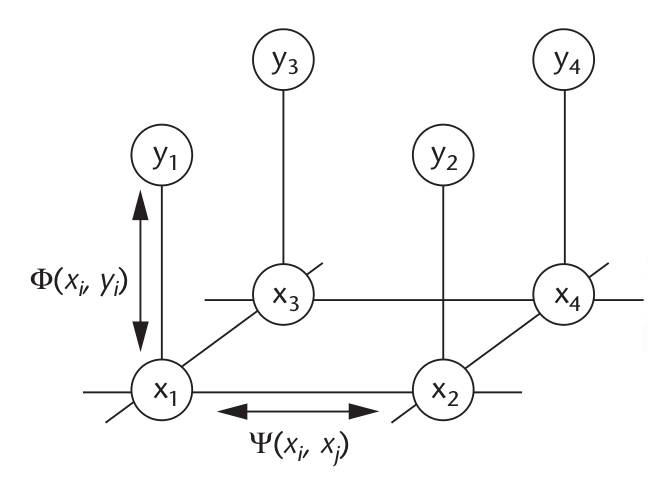
\includegraphics[scale=.5]{figs/markov}
\captionof{figure}{Markov Network}\label{markov}
\end{center}

Each vertex in the network corresponds to a patch. The conditional probability of such a joint assignment is defined as follows:
$$P(\{x_i\} | \{y_i\}) \propto \prod_{\text{neighboring } i, j} \psi(x_i, x_j) \prod_{x_i} \phi(x_i, y_i).$$

(Notice we overload “$x_i$” to mean both the vertex $x_i$ in the picture above as well as any of its candidate assignments.)
Formally we then wish to compute $\argmax_{\{x_i\}} P(\{x_i\} | \{y_i\})$.

Belief propagation is an iterative method where we make educated guesses for the $x_i$ based on their likelihood given 1) their neighbors (measured by $\psi$) and 2) their corresponding $y_i$ (measured by $\phi$). In each iteration, every node $x_i$ tell its neighbors how likely it thinks their assignments are weighted by how likely it thinks its own assignments are. This message from $x_i$ to $x_j$ (which is initialized to 1 and then normalized) is mathematically defined as follows:
$$m_{i \to j}(x_j) \propto \sum_{x_i} \psi(x_i, x_j) \phi(x_i, y_i) \prod_{k \in N_i \setminus \{j\}} m_{k \to i}(x_i)$$
(where $N_i$ is the set of neighbors of node $x_i$.) In our case this message will be a vector with an entry (a probability) for every candidate patch $x_j$ for the corresponding neighbor. Each node then uses this new information to recompute its set of messages.

To actually compute the marginal probability of each patch assignment, we define the belief of $x_i$ as follows:
$$b_i(x_i) \propto \phi(x_i, y_i) \prod_{k \in N_i} m_{k \to i}(x_i).$$
The algorithm iterates until the beliefs converge, then picks the best patch set by selecting patches that maximize the beliefs.
\subsection{Example Results}
Figure \ref{examples} gives a result from the original paper. The super-resolution algorithm is shown to be effective, even with a generic training set.
\begin{center}
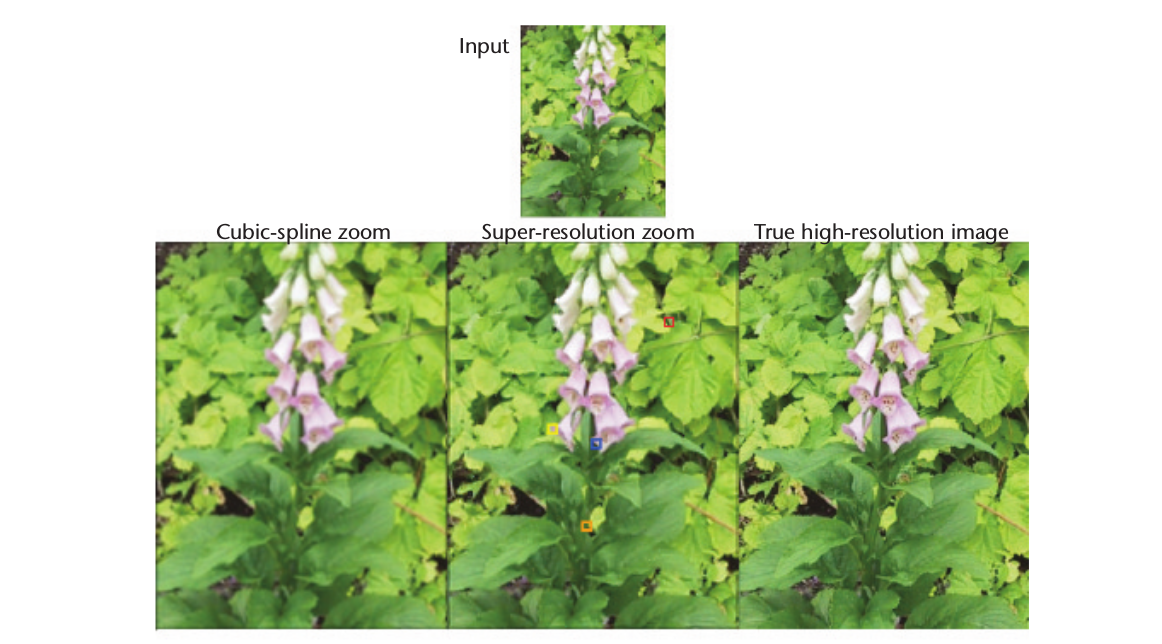
\includegraphics[scale=.4]{figs/flower}
\captionof{figure}{Markov Network}\label{examples}
\end{center}

\section{Parallel Implementation}
\subsection{Overview}
The algorithm requires a significant amount of image maniputation to the input image and the training set images.  This manipulation is not specifically a part of the belief propagation algorithm.  Due to the ease of manipulating images in Python, preprocessing and postprocessing scripts were written in Python to facilitate creating the patches for the input image and training set for use by the Charm++ belief propagation code.

\subsection{Preprocessing}
The preprocessing script was used to build the training set and output it in a convenient form. The script took as input a list of image filenames. Then for each file, it added patch pairs to the training set as follows:
\begin{enumerate}
		\item Blur, subsample, cubic-spline interpolate, high-pass filter, chunk, and contrast normalize the image to create low-frequency patches.
		\item High-pass filter, chunk, contrast normalize the image to create high-frequency patches.
		\item Append the patches in corresponding (low, high) pairs to the file containing the training set.
\end{enumerate}
Preprocessing was also done on the input image that was to be upsampled. The steps for processing an input image are as follows:
\begin{enumerate}
	\item Upsample, high-pass filter, chunk, and contrast normalize the image.
	\item Output input patches to a file.
\end{enumerate}

\subsection{Belief Propagation}
The parallel flow of the Charm++ code is given in Figure \ref{parallel} and detailed below.
\begin{center}
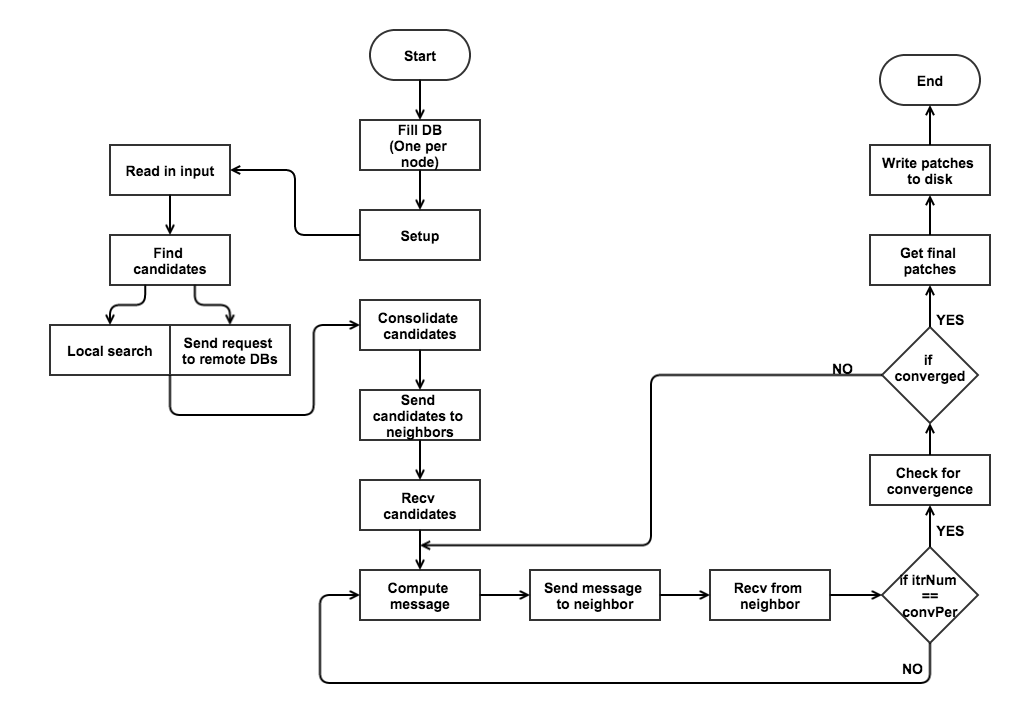
\includegraphics[scale=.4]{figs/flow}
\captionof{figure}{Parallel Flow}\label{parallel}
\end{center}

\textbf{Parallel Program Details:}
\begin{enumerate}
\item Each element in a 2-D chare array is assigned an input patch.
\item The training set will be stored in a node group. Each chare can get a pointer to the training set from the node group. Since the operations on the training set are read-only, we do not have to take care of any synchronization issues.
\item Each chare then proceeds to find the candidate patches corresponding to its input patch from the training set. Initially, this was implemented as a brute-force search. We found that this search was a signifcant bottleneck for the application. Because of this, we changed to a distributed search based locally on locality-sensitive hashing, which is further described in the \textbf{Optimizations} section below.
\item Once each chare gets its collection of candidate patches, it sends these candidates to its neighbors. After receiving the patches from its neighbors, each chare calculates $\psi$ and $\phi$. This calculation needs to be done only once as the candidate patches do not change between iterations. This completes the setup phase of chares.
\item In each iteration, the chares compute the message $m_{ij}$ for each candidate patch of the neighbors. Once the messages are calculated they are sent to each of the neighboring chares, which use them to update their own outgoing messages. Finally, a convergence test is performed by calculating the belief for each of the candidate patches, creating an array of beliefs (one per candidate patch.) This convergence test is done at the end of every $n$ iterations, where $n$ was taken to be five for our test runs.
\item To test for convergence, we will examine the change in the beliefs between iterations. This will be computed as an element-wise difference between the belief array for the current iteration and the previous iteration on each chare. Then, the $\ell^2$-norm of the array of the change in the beliefs between iterations will be computed. A max reduction will then be performed and the main chare will compare the max $\ell^2$ norm of the changes to a specified tolerance. If the maximum change is less than the specified tolerance, the results will be reduced to the main chare, which will output the resulting patches and exit. Otherwise, the main chare calls an entry method on the chare array to begin the next iteration.
\end{enumerate}

\subsection{Postprocessing}
The Python script for postprocessing takes the original input image and the patches outputted by the Charm++ code as input. The input image is upsampled using a cubic-spline interpolation. The algorithm then contrast denormalizes the patches and adds each patch to the appropriate place in the upsampled image.

\subsection{Optimizations}
The brute-force search that was originally used to find candidates was a major bottleneck. Two optimizations were made to improve the search.  First, the brute-force search was replaced by a locality-sensitive hashing search. This is an approximate search method in which we want similar items to hash into the same bin with high probability. We used the implementation available in the LSHBOX library. Then, we moved from a local search to distributed search.

The distributed search makes use of node groups for efficiency. Each node group shares a complete copy of the training database as originally designed. However, every node group is responsible for searching only a subsection of the database. So, to get good candidate patches from throughout the database a chare follows this process:
\begin{enumerate}
\item Request more candidates from the other node groups.
\item Search for candidates in the local part of the database.
\item Prune the candidate set down to $num$ items, where $num$ was $16$ for our tests.
\end{enumerate}
The request for more candidates from a remote node group can be fulfilled by any chare in the specified node group, depending on which chares are available for work.

\subsection{Multiple Input Images}
In order to handle multiple images we replicate the chare array responsible for the steps \textbf{Find candidates} through \textbf{Get final patches} in Figure \ref{parallel}. The arrays (each uniquely indexed) run entirely separately from one another since we make the simplifying assumption that the images are independent. This can generate load imbalance since different images might converge at different steps, either because they have different sizes or because they are of a different complexity. The final reductions (in steps \textbf{Check for convergence} and \textbf{Get final patches}) are tagged with the particular array's index to ensure its chosen patches are saved in the proper files (if converged) or run another belief propagation iteration (if not yet converged).

In practice, the code would likely be run on a sequence of images with temporal continuity (such as a video stream), in which case the network in Figure \ref{markov} could be extended to have a 3D $\{x_i\}$ grid, increasing both computation and communication.

\section{Results}
The following sections illustrate both the physical results and the parallel results for the implemented project.
\subsection{Image Results}
The actual image resulting from our implementation and the standard cubic-spline interpolation are illustrated in Figure \ref{lenna}.  The left image illustrates the result of using cubic-spline interpolation to upsample the image.  The right image illustrates the result of the our implementation.  The right image is more visibly blocked than desired.  This is due to contrast normalization issues.  In the papers by \citet{fjp} and \citet{fp}, it was specified that the input patches and training set patches were contrast normalized and the ouptut patches were contrast denormalized.  However, the exact method of contrast normalization and denormalization was not specified.  We were unable to determine the method they used and the method of normalization we used resulted in the somewhat blocked appearance of the super-resolution image shown on the right in Figure \ref{lenna}. 

\begin{figure}[ht!]
\centerline{%
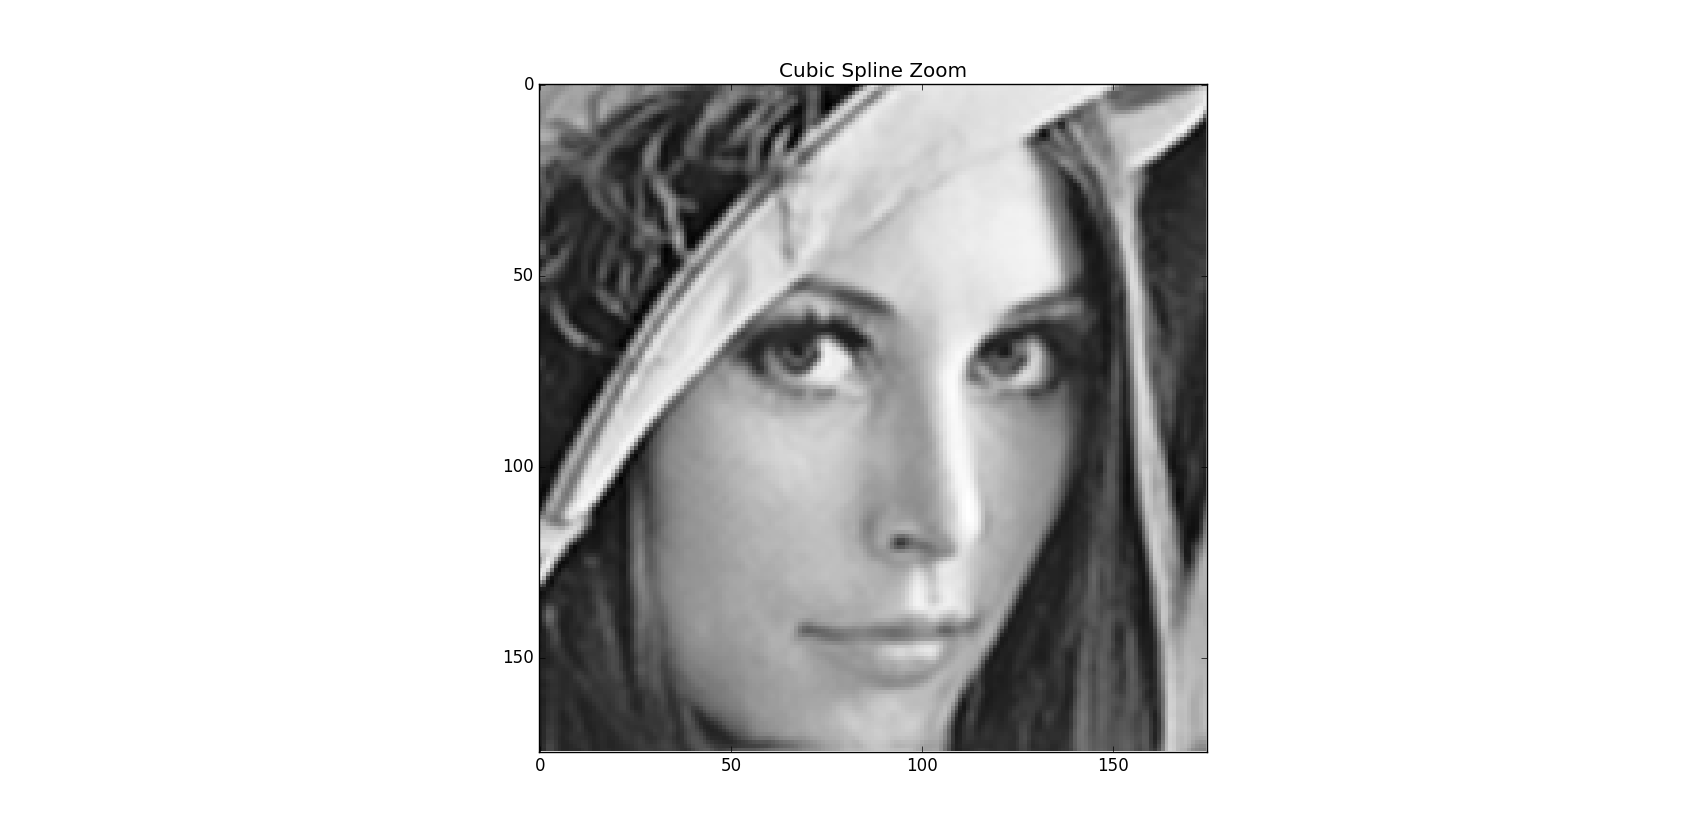
\includegraphics[width=0.5\textwidth]{figs/cubic-spline-zoom}%
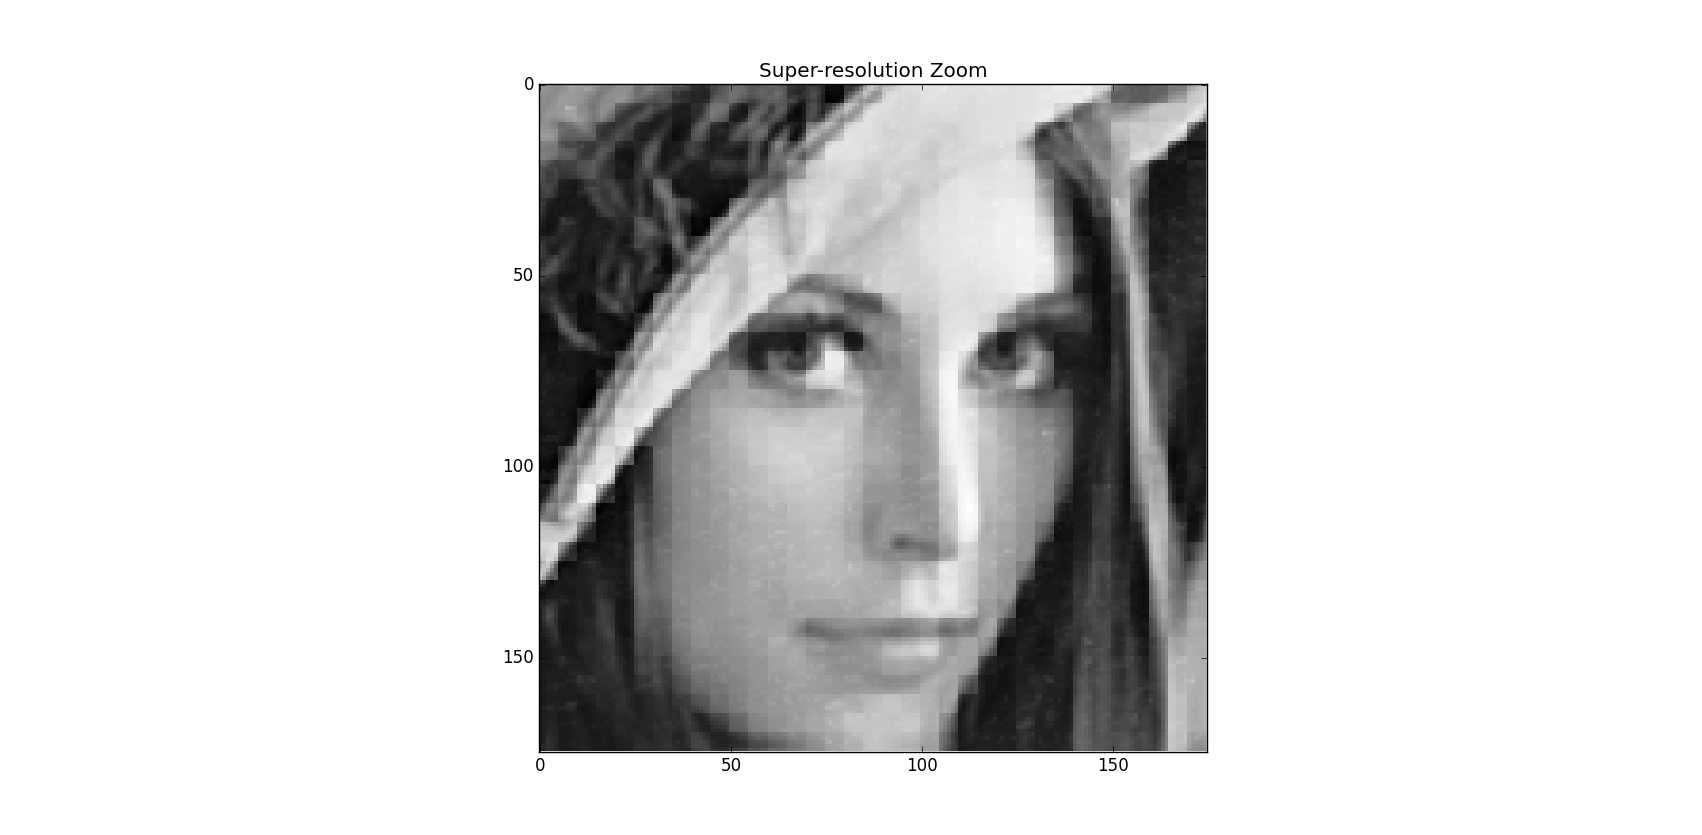
\includegraphics[width=0.5\textwidth]{figs/super-res-zoom}%
}%
\caption{Our Implemenation Output}
\label{lenna}
\end{figure}


\subsection{Parallel Performance Results}
Strong scaling of the Charm++ code was evaluated for a couple of database sizes and input image sizes.  Specifically, the code was run for two different database sizes: BigDB (793121 patches) and SmallDB (13268 patches), and two different input image sizes:  BigImage (43200 patches) and SmallImage (1225 patches).  The strong scaling results for each of the possible combinations of image size and database size are shown in Figure \ref{scalability}.  Each graph shows a log-log plot of the full application time, database load/setup time (DB load), and the compute time.  The compute time is the time to search the DB and perform the parallel belief propagation, but does not include the database load/setup time.  Each graph also includes a line that shows linear scaling for comparison.  It is important to note that each of the graphs were obtained via different runs on Taub, so the actual timing results may not be consistent across runs, but the general trends within a plot should be somewhat consistent.

The first row of Figure \ref{scalability} illustrates the results with SmallDB.  Examining these graphs, it is seen that the DB load time was a large portion of the actual time.  Up through 64 cores, scaling was close to linear for DB load, full application and compute times.  However, at 128 cores, it hit a scaling limit.  This is likely due to a large amount of out of node communication.  This is seen for both the small image size and large image size, but is significantly more pronounced for the small image.  For the small image, the time actually increased when going up to 128 cores, likely because of too much parallel overhead to computation.

The second row of Figure \ref{scalability} illustrates the results with BigDB.  Examining the second row, it is seen that with the BigDB, the time to load/setup the DB was almost all of the full application time. This is a result of the fact that the search method for the database utilizes machine learning, and the training of the database search (not the actual search) is included as database setup time.  Despite our optimizations, this is still a significant factor in execution time.  Looking at the slope of the line for DB load and full application, it can be seen that superlinear scaling was achieved.  This is likely a result of the fact that the database load time increases at a faster than linear rate as the database size increases.  Since increasing the number of cores decreases the size of the database for which each core is responsible, superlinear scaling is achieved for both DB load and full application.  Examining only the compute time for the second row, it is seen that scaling was almost exactly linear for the compute time which includes the actual distributed search time and the belief propagation time.

\begin{figure}[ht!]
\centerline{%
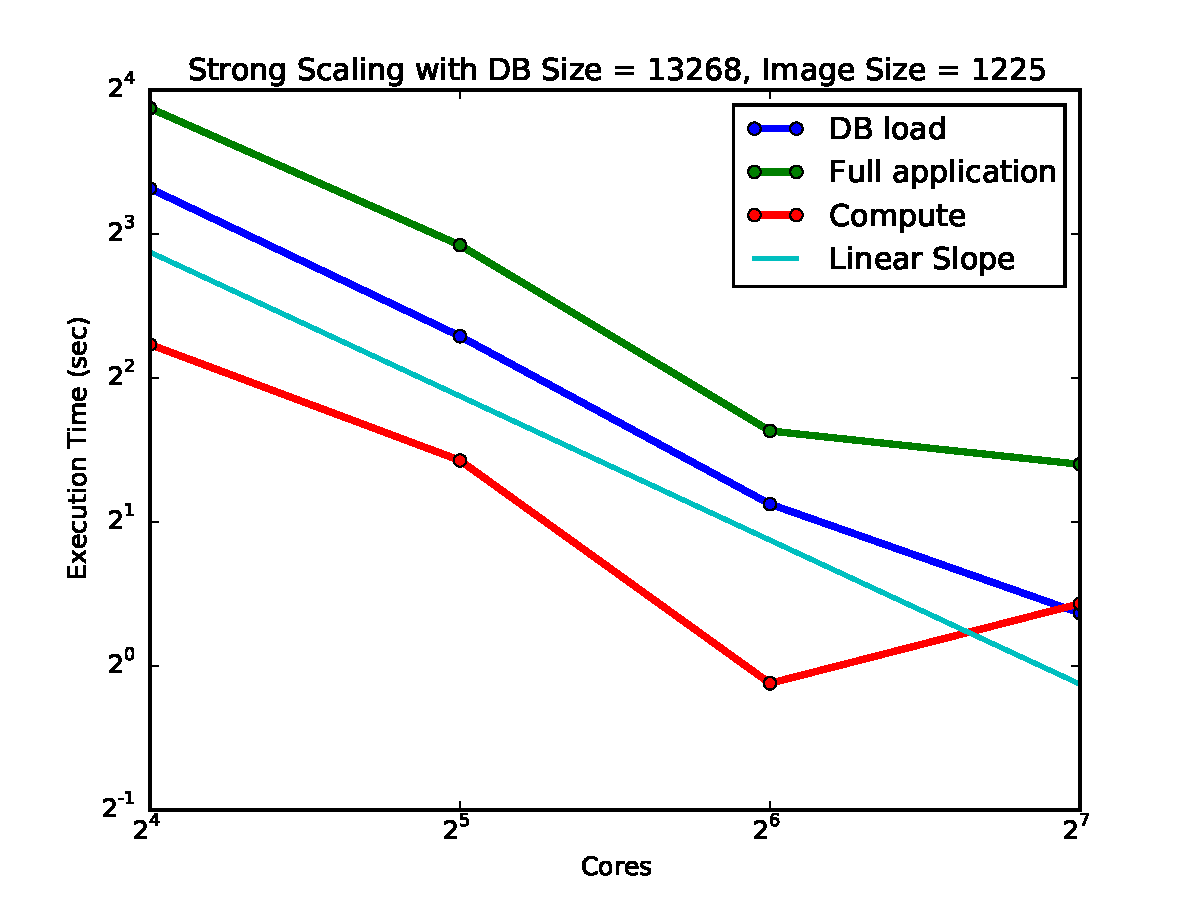
\includegraphics[width=0.5\textwidth]{figs/13268_1225}%
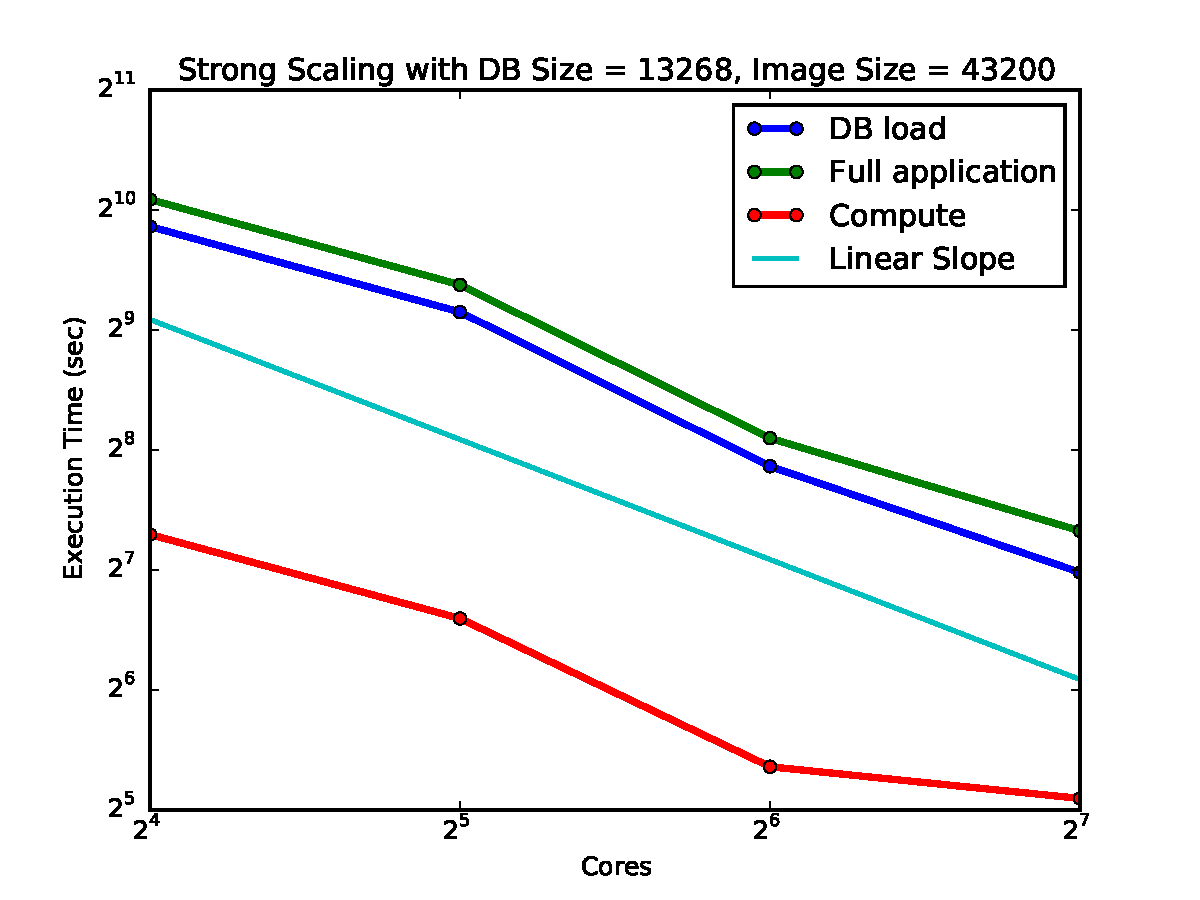
\includegraphics[width=0.5\textwidth]{figs/13268_43200}%
}%
\centerline{%
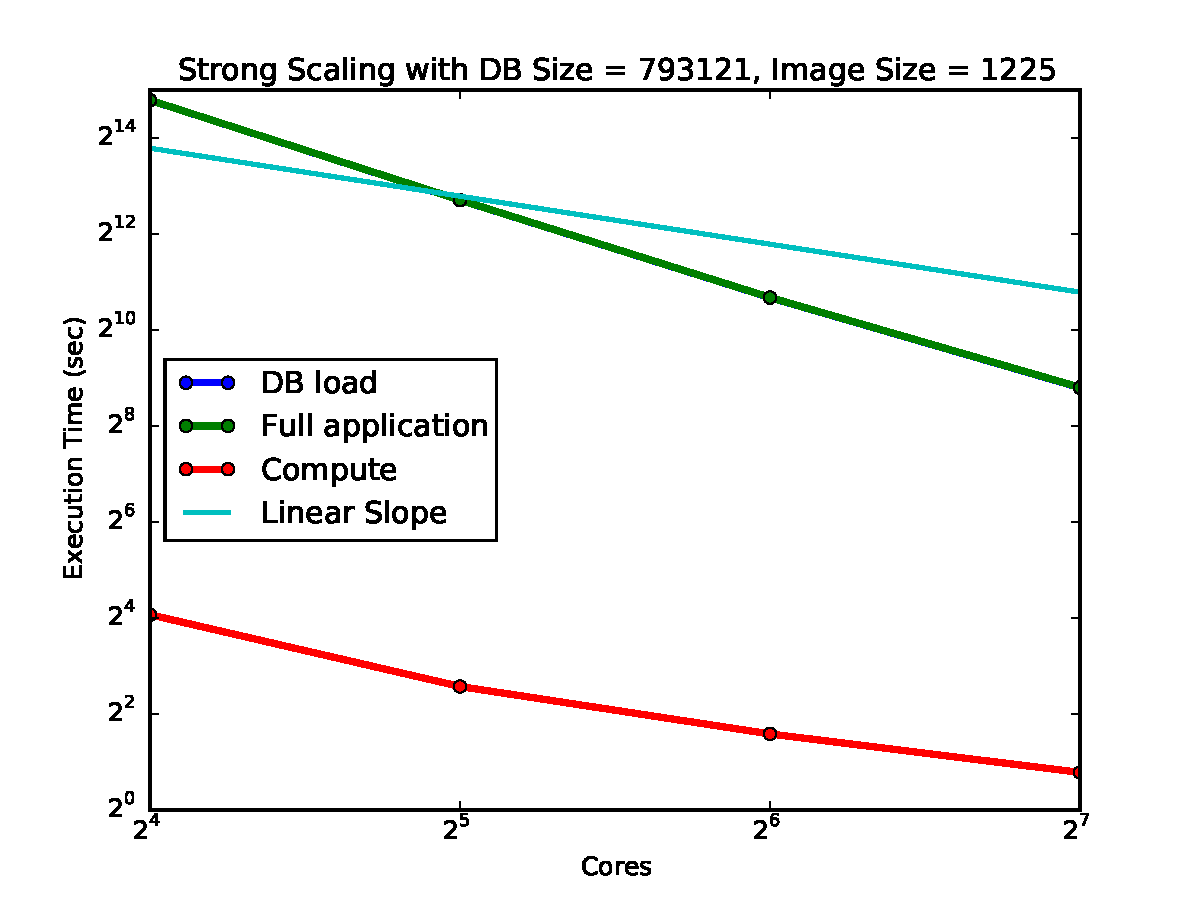
\includegraphics[width=0.5\textwidth] {figs/793121_1225}%
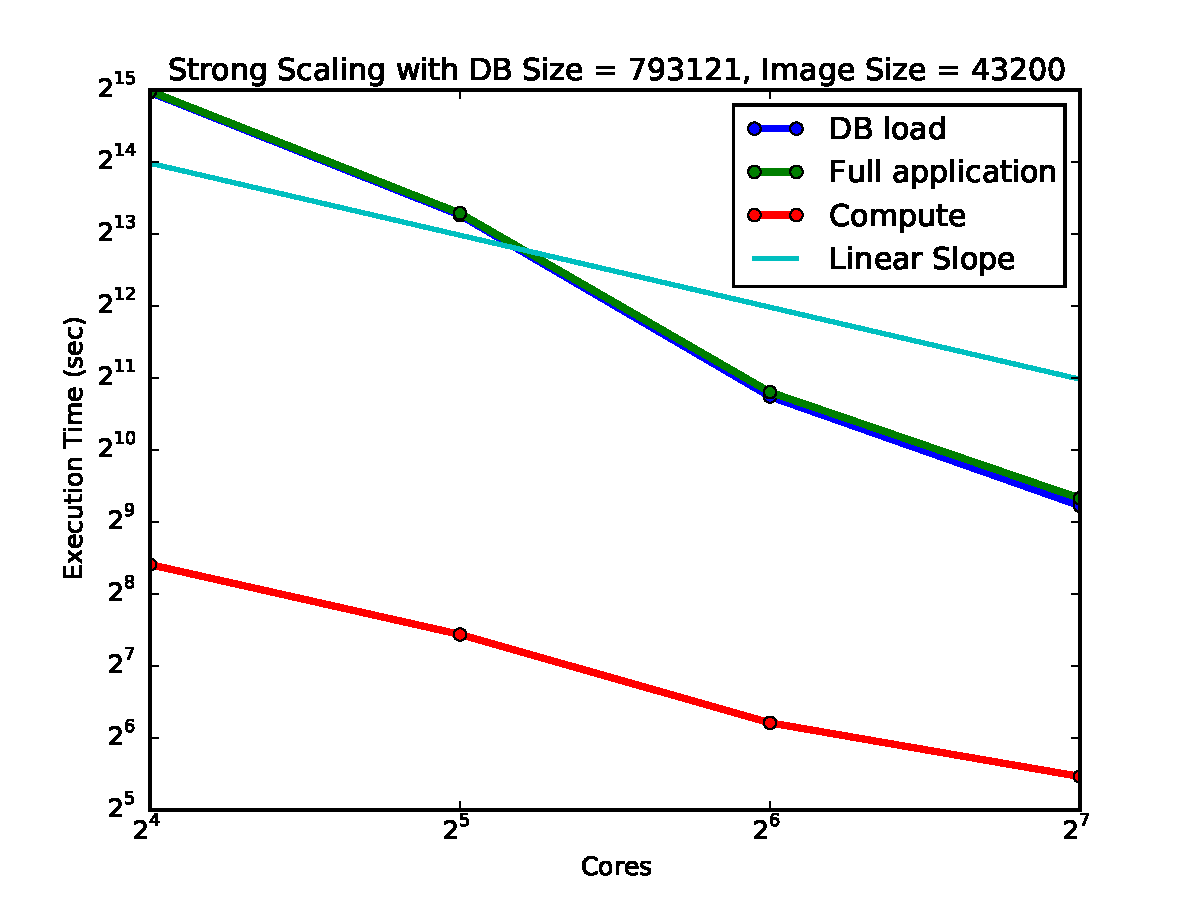
\includegraphics[width=0.5\textwidth] {figs/793121_43200}%
}%
\caption{Strong Scaling Results}
\label{scalability}
\end{figure}

In addition to the performance results presented above, strong scaling of the Charm++ code was also evaluated for multiple input images.  This was only run with the SmallDB due to time constraints and the large amount of input images being processed.  Figure \ref{scale_multi} shows the strong scaling results for this test case.  Examining this, it is seen that even almost exactly linear scaling was achieved for DB load, full application, and compute.  Additionally, it is also seen that this did not suffer the same scalability hit as the results from using the SmallDB.  This is likely due to the fact that the overall work computation increased, so the parallel overhead was not as significant.

\begin{center}
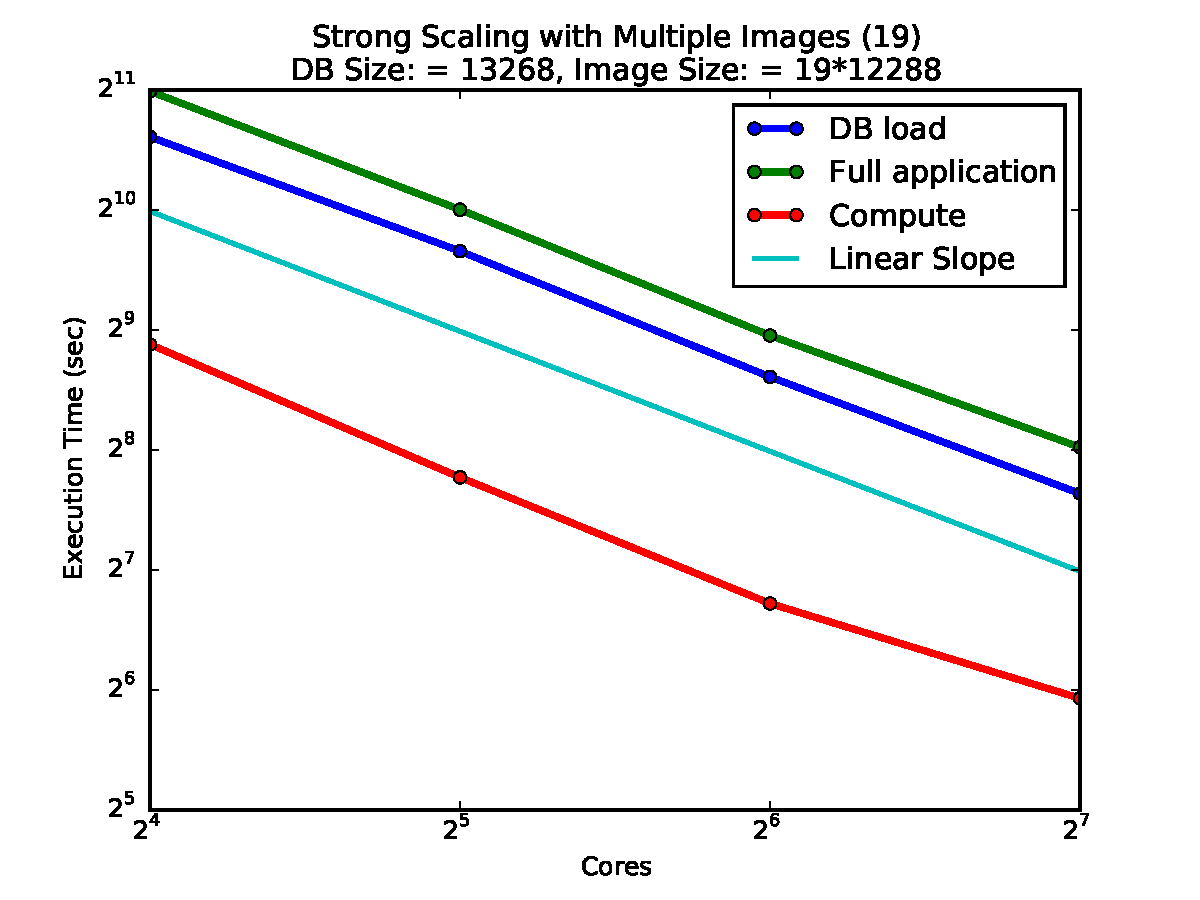
\includegraphics[scale=.4]{figs/13268_19_12288}
\captionof{figure}{Strong Scaling with Multiple Images}\label{scale_multi}
\end{center}

In addition to examining the scaling of the parallel implementation, Projections was also utilized to determine if load-balancing was needed.  Theoretically, the load should be well distributed as each chare has almost the same amount of computation and communication, with the only deviation being that the chares with the edge patches have slightly less.  Figure \ref{projections} illustrates the projections results.  From this, it is seen that almost all of the processors are equally utilized and none of the processors are over-utilized, indicating that load-balancing is not necessary.

\begin{center}
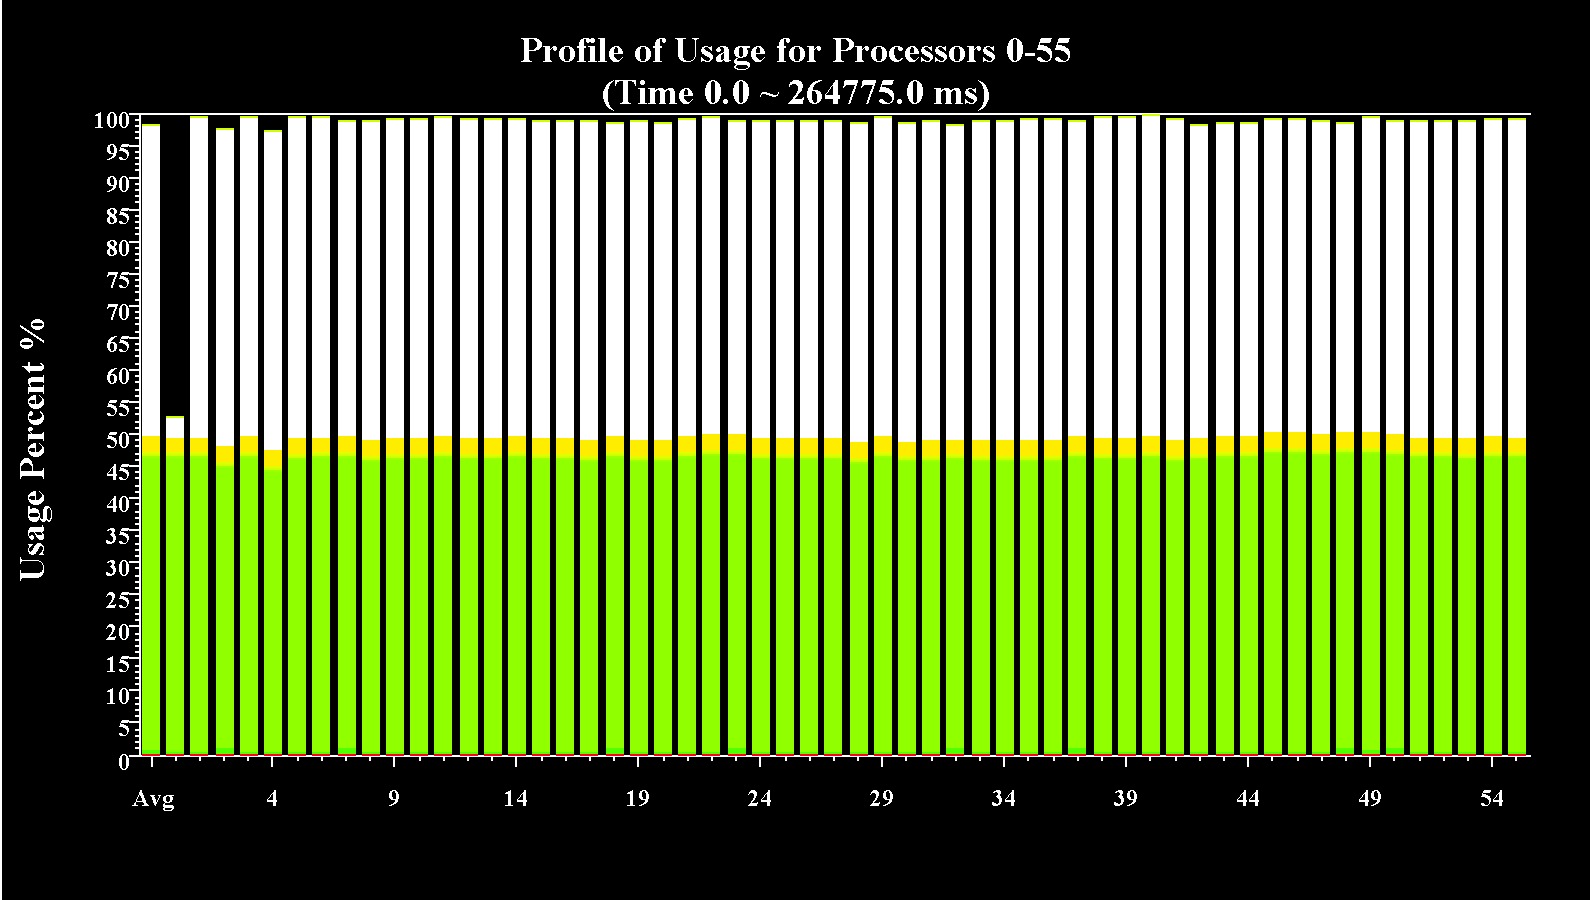
\includegraphics[scale=.4]{figs/projections_results}
\captionof{figure}{Projections}\label{projections}
\end{center}

Furthermore, we also utilized Projections when running with multiple input images to determine if the multiple input images presented a load-balancing issue.  Figure \ref{projections_multi} illustrates the projections results before load-balancing (left) and after load-balancing (right).  Examining these, it is seen that the without load-balancing, there is some load imbalance, seen by the height difference between the far left processors and far right processors.  The result on the right illustrates the results with RefineLB load balancer which was able to remedy a decent portion of the load imbalance.

\begin{figure}[ht!]
\centerline{%
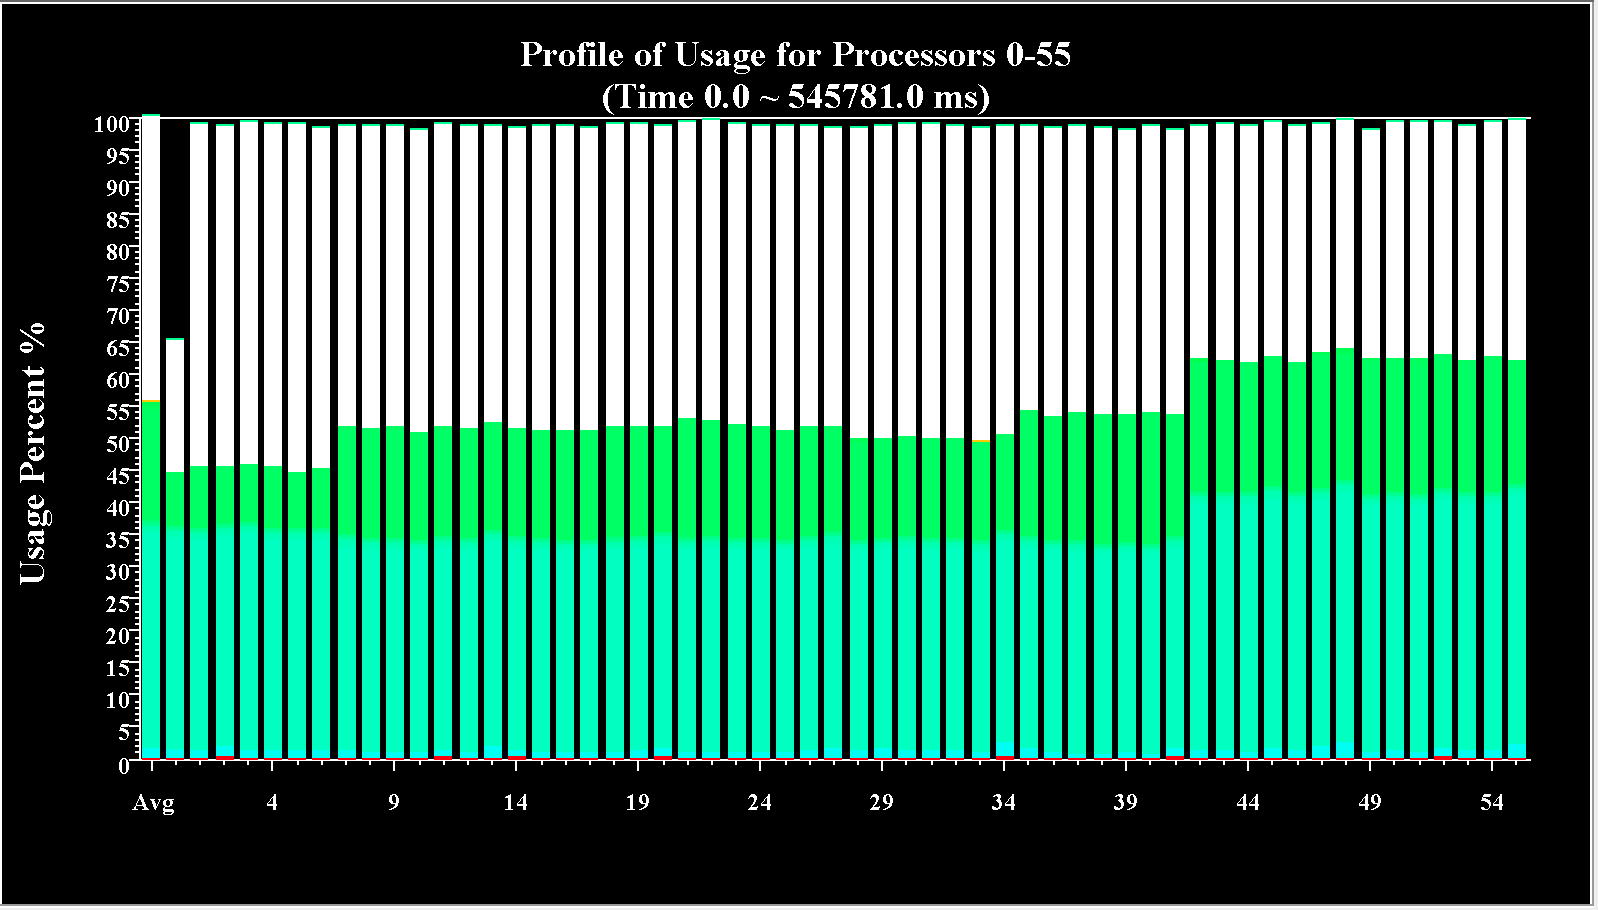
\includegraphics[width=0.5\textwidth]{figs/multi_nobalance}%
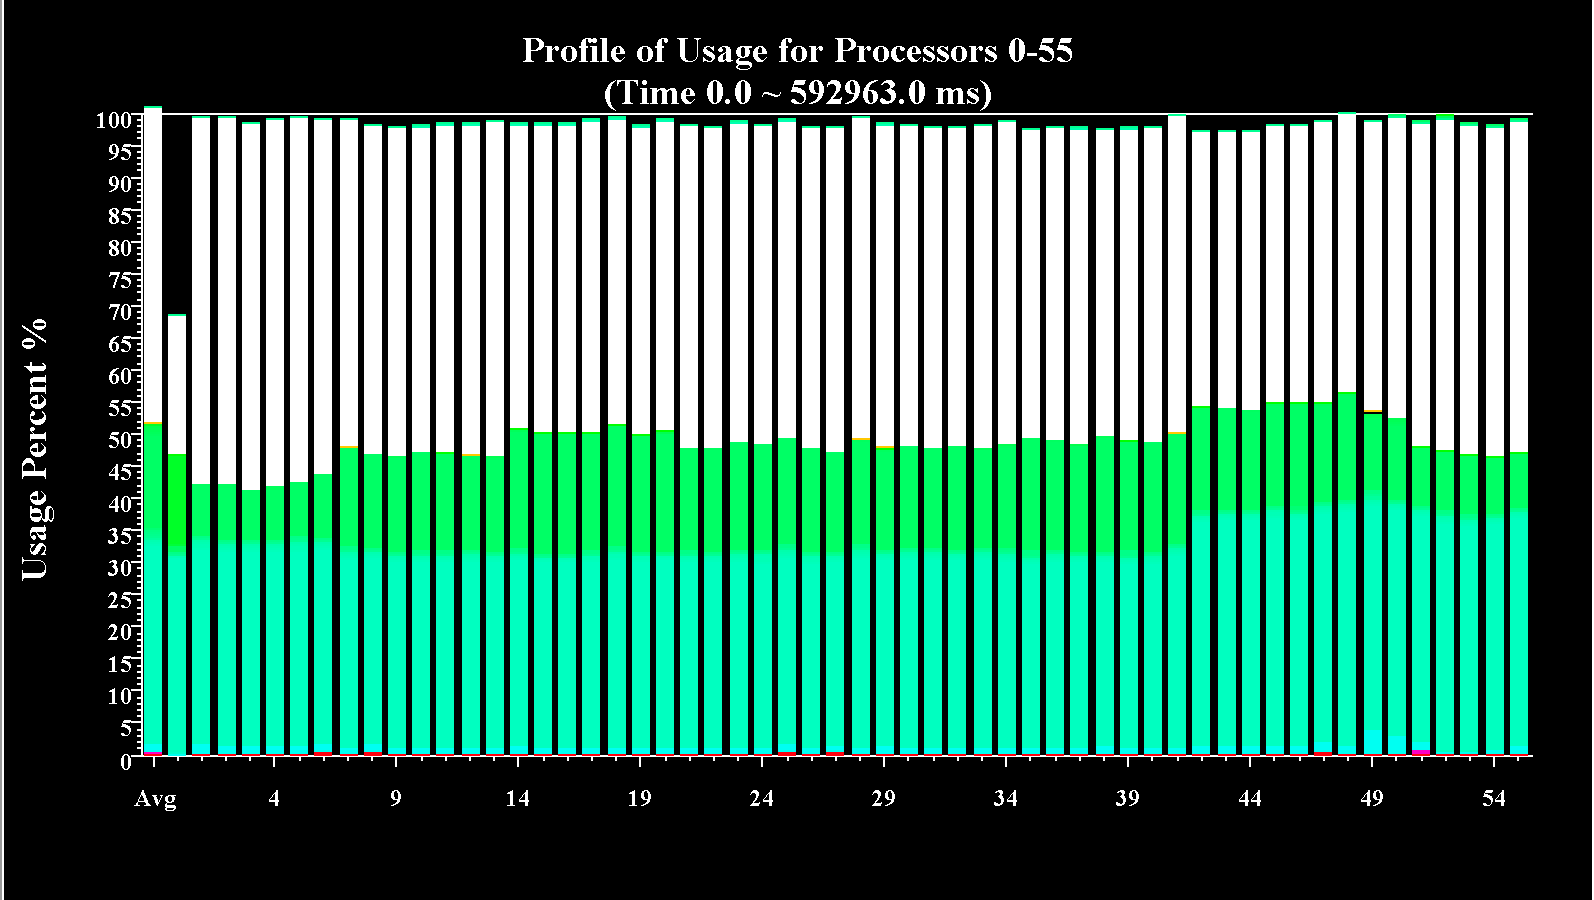
\includegraphics[width=0.5\textwidth]{figs/multi_balance}%
}%
\caption{Projections for Multiple Images}
\label{projections_multi}
\end{figure}

\section{Conclusion}
This project implemented parallel belief propagation for image super-resolution using a distributed database with an integrated locality-sensitive hashing search.  Additionally, preprocessing and postprocessing was implemented in Python scripts.  Physical results, scalability results, and Projections results were presented illustrating the performance of the implemented project.  Had time permitted, investigating an even better database search (with a smaller load/setup time) could have obtained even better results as this was still the bottleneck in the application.  However, even as is, we were able to obtain good strong scaling results when using the BigDB.

\bibliographystyle{plainnat}
\nocite*{}
\bibliography{bibentries.bib}

\end{document}